\documentclass[tikz,border=10pt]{standalone}
\usepackage{tikz}
\usetikzlibrary{arrows.meta,decorations.pathmorphing,calc}

\begin{document}
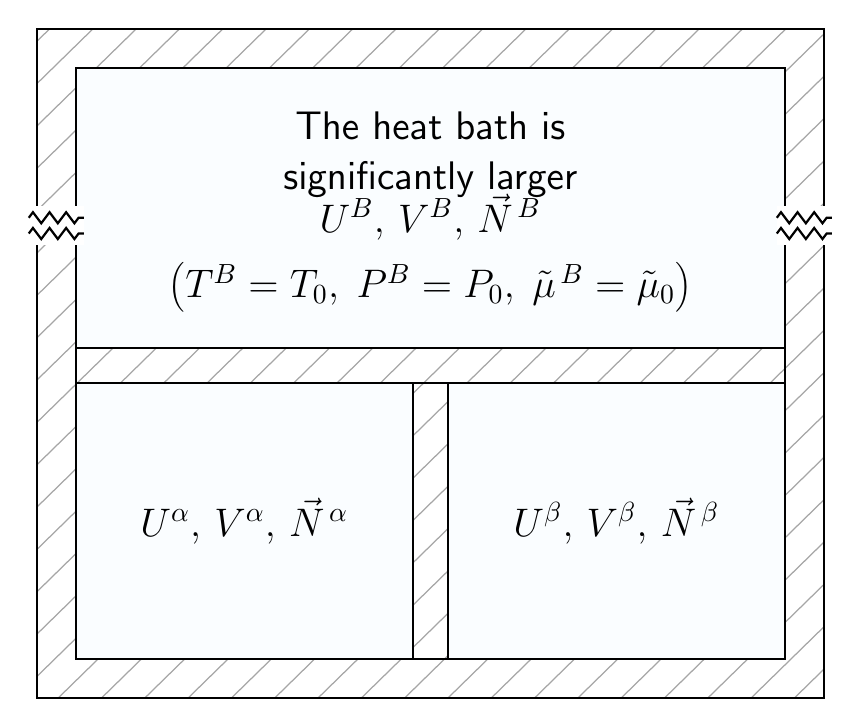
\begin{tikzpicture}
    % --- Dimensions ---
    \def\TotalW{10}        % Total Width
    \def\TotalH{8.5}       % Total Height
    \def\WallThick{0.5}    % Insulation thickness (outer ring)
    \def\BandH{0.45}       % Thickness of the internal horizontal wall band
    \def\SepY{4.0}         % Bottom y of the horizontal band
    \def\MidWallW{0.45}    % Thickness of the vertical middle wall
    \def\BreakY{6.0}       % y-location of side "break" zigzags

    % --- Derived positions ---
    \pgfmathsetmacro{\InnerL}{\WallThick}
    \pgfmathsetmacro{\InnerR}{\TotalW-\WallThick}
    \pgfmathsetmacro{\InnerB}{\WallThick}
    \pgfmathsetmacro{\InnerT}{\TotalH-\WallThick}
    \pgfmathsetmacro{\MidX}{\TotalW/2}
    \pgfmathsetmacro{\BandTop}{\SepY+\BandH}
    \pgfmathsetmacro{\MidWallL}{\MidX-\MidWallW/2}
    \pgfmathsetmacro{\MidWallR}{\MidX+\MidWallW/2}

    % --- Styles ---
    \tikzset{
        gas style/.style={
            fill=cyan!2,
            draw=black,
            thick
        },
        break line/.style={
            thick,
            decorate,
            decoration={zigzag, amplitude=2pt, segment length=6pt}
        },
        math text/.style={font=\Large},
        label text/.style={font=\sffamily\Large, align=center}
    }

    % =========================================================
    % 1) BACKGROUND HATCH (clipped to the OUTER box only)
    % =========================================================
    \begin{scope}
      \clip (0,0) rectangle (\TotalW,\TotalH);

      \def\HatchStep{0.55} % adjust density: smaller = denser
      \foreach \t in {-80,...,140} {
        \draw[gray!70, line width=0.45pt]
          (-12+\t*\HatchStep, -12) -- (-12+\t*\HatchStep+45, 32);
      }
    \end{scope}

    % Outer border
    \draw[thick] (0,0) rectangle (\TotalW,\TotalH);

    % =========================================================
    % 2) GAS REGIONS (these "erase" hatch where placed)
    % =========================================================

    % --- TOP HEAT BATH GAS REGION ---
    \filldraw[gas style]
      (\InnerL, \BandTop) rectangle (\InnerR, \InnerT);

    % --- BOTTOM LEFT BOX (alpha) ---
    \filldraw[gas style]
      (\InnerL, \InnerB) rectangle (\MidWallL, \SepY);

    % --- BOTTOM RIGHT BOX (beta) ---
    \filldraw[gas style]
      (\MidWallR, \InnerB) rectangle (\InnerR, \SepY);

    % =========================================================
    % 3) OUTLINES FOR INTERNAL HATCHED WALLS
    %    (We do NOT fill them; hatch already exists underneath.)
    % =========================================================

    % Inner cavity border (gives the "ring" look)
    \draw[thick] (\InnerL,\InnerB) rectangle (\InnerR,\InnerT);

    % Horizontal band (hatched automatically)
    \draw[thick] (\InnerL,\SepY) rectangle (\InnerR,\BandTop);

    % Vertical middle wall (hatched automatically)
    \draw[thick] (\MidWallL,\InnerB) rectangle (\MidWallR,\SepY);

    % =========================================================
    % 4) SIDE BREAK ZIGZAGS (same trick as before)
    % =========================================================
    % --- LEFT BREAK ---
    \fill[white] (-0.1, \BreakY-0.25) rectangle (\WallThick+0.1, \BreakY+0.25);
    \draw[break line] (-0.1, \BreakY+0.1) -- (\WallThick+0.1, \BreakY+0.1);
    \draw[break line] (-0.1, \BreakY-0.1) -- (\WallThick+0.1, \BreakY-0.1);

    % Restore vertical border lines
    \draw[thick] (0, \BreakY+0.25) -- (0, \TotalH);
    \draw[thick] (0, 0) -- (0, \BreakY-0.25);
    \draw[thick] (\WallThick, \BreakY+0.25) -- (\WallThick, \TotalH-\WallThick);
    \draw[thick] (\WallThick, \WallThick) -- (\WallThick, \BreakY-0.25);

    % --- RIGHT BREAK ---
    \fill[white] (\TotalW-\WallThick-0.1, \BreakY-0.25) rectangle (\TotalW+0.1, \BreakY+0.25);
    \draw[break line] (\TotalW-\WallThick-0.1, \BreakY+0.1) -- (\TotalW+0.1, \BreakY+0.1);
    \draw[break line] (\TotalW-\WallThick-0.1, \BreakY-0.1) -- (\TotalW+0.1, \BreakY-0.1);

    % Restore vertical border lines
    \draw[thick] (\TotalW, \BreakY+0.25) -- (\TotalW, \TotalH);
    \draw[thick] (\TotalW, 0) -- (\TotalW, \BreakY-0.25);
    \draw[thick] (\TotalW-\WallThick, \BreakY+0.25) -- (\TotalW-\WallThick, \TotalH-\WallThick);
    \draw[thick] (\TotalW-\WallThick, \WallThick) -- (\TotalW-\WallThick, \BreakY-0.25);

    % =========================================================
    % 5) TEXT
    % =========================================================

    % Title in heat bath
    \node[label text] at (\MidX, \InnerT - 1.1) {
        The heat bath is \\ significantly larger
    };

    % Heat bath variables + constraints
    \node[math text, align=center] at (\MidX, \BandTop + 1.2) {
        $U^B,\, V^B,\, \vec{N}^{\,B}$\\[2mm]
        $\left(T^B=T_0,\; P^B=P_0,\; \tilde{\mu}^{\,B}=\tilde{\mu}_0\right)$
    };

    % Bottom left (alpha)
    \node[math text] at ({(\InnerL+\MidWallL)/2}, {(\InnerB+\SepY)/2}) {$U^\alpha,\, V^\alpha,\, \vec{N}^{\,\alpha}$};

    % Bottom right (beta)
    \node[math text] at ({(\MidWallR+\InnerR)/2}, {(\InnerB+\SepY)/2}) {$U^\beta,\, V^\beta,\, \vec{N}^{\,\beta}$};

\end{tikzpicture}
\end{document}